% Etiquetas que uso para editar en la próxima iteración:
% FALTA, VER


\chapter{ \textsc{ Diseño Digital } }\label{CONAMURI}

\textsl{ Bla bla bla bla bla bla bla ...\footnote{ Un groso } } 

%\vspace{10mm}

%\textbf{Por Magui Balbuena}\footnote{ Maguiorina (Magui) Balbuena  es dirigente de CONAMURI }

\vspace{10mm}

\section{Introducción}
Es importante lograr sumadores binarios rápidos y eficientes según el uso de área y potencial La suma es la operación elemental para lograr otras operaciones muy utilizadas en los circuitos aritméticos. Ejemplo de esto son los multiplicadores, la resta, división, los filtros FIR e IIR, por nombrar las más conocidas.

%FIGURA
%(Multiplicadores, Filtros FIR, usando sumadores)

Para cada una de esas operaciones, son necesarios sumadores de distinta cantidad de bits en el mismo diseño. Por lo cuál, no se trata solamente de encontrar la arquitectura que para una determinada cantidad de bits logre el mejor compromiso de área, potencia y velocidad. Sino también lograr una relación de compromiso según crece la cantidad de bits del sumador. 

\subsection{Semisumador y sumador completo}
\subsubsection{Semisumador}
El {\bf Semisumador} (Half-adder) recibe 2 bits de entradas \(a\) y \(b\) y produce un bit de suma \(s= a \oplus b\) y un bit de acarreo \(c= a b\).

\subsubsection{Sumador Completo}
Luego definimos un Sumador Completo de un bit, o Full Adder:
\begin{center}
\begin{tabular}{lll}
Entradas: & Bits de operandos \(a\) , \(b\) y carry-in \(c_{in}\) & (o \(x_i, y_i, c_i\) para la etapa \(i\)) \\
Salidas: & Suma \(s\) y carry-out \(c_{out}}\) & (o \(s_i\) y \(c_{i+1}\) para la etapa \(i\)) \\
\end{tabular}
\end{center}


\(s=x\oplus y \oplus c_{in}

%\(c_{out}= (a\wedge b )\vee (a \wedge c_{in}) \vee (b\wedge c_{in})\)

\(c_{out}= a b + a c_{in} + b c_{in}\)

Podemos construir un {\bf sumador completo} (full-adder) a partir del semisumador, como vemos en la siguiente figura:

\vspace{-1pt}

\begin{figure}[h]
  \centering
\begin{subfigure}[b]{0.3\textwidth}
                \centering
                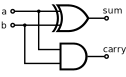
\includegraphics[width=\textwidth]{figuras/halfadd_schem.pdf}
                \caption{[Semisumador]}
                \label{fig:halfadder}
        \end{subfigure}
\begin{subfigure}[b]{0.3\textwidth}
                \centering
                \includegraphics[scale=0.95]{figuras/fullAdd.pdf}
                \caption{[Sumador completo]}
                \label{fig:fulladder}
        \end{subfigure}

  \caption{Bit adders}\label{fig:bitadders}

\end{figure}

\vspace{0.5cm}



\section{Selección de la arquitectura del sumador}

Proponemos el uso de Celdas estándard CMOS (Complementary Metal Oxide Silicon) para la implementación\footnote{Para ver otras posibilidades de implementación lógica, ver (FALTA CITA) RABAEY}. El carácter de nuestro flujo de diseño así lo requiere, ya que se utilizarán herramientas de síntesis de circuitos digitales basadas en celdas estándars. Quedan entonces descartadas las implementaciones utilizando transmition gates, lógica dinámica u otro tipo de implementacion lógica.

\subsection{Costo y Retardo de los circuitos combinacionales}
Cada circuito combinacional \(G\) tiene un costo y un retardo. El costo de un circuito combinacional es la suma de los costos de las compuertas en un circuito. Le asignamos un costo unitario a cada compuerta, y el costo del circuito combinacional \(c(G)\) es igual al número de compuertas en el circuito.

El retardo de un circuito combinacional \(d(G)\) se define igual al del retardo de una compuerta. Es el menor tiempo requerido para que las salidas se estabilicen, asumiendo que todas las entradas están estables. Para simplificar el análisis, se le asigna un retardo unitario a cada compuerta.



\subsection{Clasificación de los sumadores}

Dentro de los sumadores paralelos, se encuentran varias arquitecturas, cada una con sus ventajas y desventajas. Hacemos una lista de algunas de ellas:

\vspace{0.3cm}

\begin{tabular}{ |l|l| }
  \hline
  \multicolumn{2}{|c|}{Sumadores Binarios} \\
  \hline

RCA & Ripple Carry Adder \\
CLA & Carry Look-Ahead Adder \\
CSkA & Carry Skeep Adder \\
CA & Canonical Adders \\
BBCLA & Block-based Look-Ahead Adders \\
CondSumA & Conditional Sum Adder \\
CSeA & Carry Select Adder \\
HybAd & Hybrid Adders \\
NPA & Network Prefixs Adders: \\
& Ladner and Fischer \\
&Kogge-Stone \\
&Brent-Kung \\
&Skalansky \\
  \hline
\end{tabular}
\vspace{0.3cm}

%Carry Save Adder (CSaA) & \(O(n) \)& \(O(\log (n)) \)\\ \hline
%Carry Skip Adder (CSA) &\( O(n) \)& \(O(n^{l+2/l+1})\) \\ \hline
%Carry Increment Adder (CIA) &\( O(n)\) &\( O(n^{l+2/l+1})\) \\ \hline

\subsubsection{Ripple Carry Adder}

Definimos el sumador Ripple Carry Adder (RCA), utilizando \(n\) full-adders para sumar 2 operandos de \(n\) bits. El sumador de \(n\) bits produce una salida de \(n\) bits y una salida de acarreo \(c_{out}\)

Este sumador se implementa conectando como muestra la figura\ref{RCA} el bloque FA (Full Adder). El camino crítico de la señal se determina considerando el peor camino de propagación de la señal.  

%\vspace{-1pt}
\begin{figure}[h]
  \centering
%  \subfloat[Half adder]
{\label{RCA}\includegraphics[scale=1.5]{figuras/binnaryAdder.pdf}}
  \caption{Riple Carry Adder}
\vspace{-10pt}
\end{figure}

Resumimos las características y diferencias entre los distintos sumadores\cite{6120598}:
%\cite{estrada-gimenez}
%Comenzamos con el RCA (Ripple Carry Adder), que tiene un área O(n) y un retardo de compuerta (Delay) de O(n).
%Luego tenemos al CLA (Carry Look-Ahead Adder) con un área de O(n*log(n)) y un delay de O(log(n)).
%Carry Skip Adder(CSA)
%Carry Increment Adder (CIA) Área O(n) y Delay O (nl + 2/ l +1 )  
%Carry Select Adder (CSelA)Área O(n) y Delay O (nl + 2/ l +1 ) 
 
% El delay de un RCA está en pag. 77 de Computer Arithmetic de Behrooz Parhami


\subsubsection{Retardo Máximo y Área de las distintas arquitecturas}
\begin{table}[t]
\caption{Resumen Características de Sumadores}
\begin{tabular}{|l|l|l|}
\hline
\multicolumn{1}{|c|}{\textbf{Arquitectura}} & \multicolumn{1}{c|}{\textbf{Retardo Máx.   }} & \multicolumn{1}{c|}{\textbf{Área}} \\ \hline
Ripple Carry Adder (RCA) & \(O(n)\) & \(O(n)\) \\ \hline
Carry Save Adder (CSaA) & \(O(\log(n)) \)& \(O(n) \)\\ \hline
Carry Look-Ahead Adder (CLA) & \(O(\log(n))\) & \(O(n\log(n))\) \\ \hline
Carry Skip Adder (CSA) &\(O(n^{l+2/l+1})  \)& \(O(n)\) \\ \hline
Carry Increment Adder (CIA) &\(O(n^{l+2/l+1})  \)& \(O(n)\) \\ \hline
Carry Select Adder (CselA) &\(O(n^{l+2/l+1})  \)& \(O(n)\) \\ \hline
Ladner-Fisher &\( O(\log(n))\) & \(O(n\log(n))   \) \\ \hline
Skalansky &\( O(n\log_2(n))\) & \(O(\log^2(n))\) \\ \hline
Kogge-Stone & \( O(n\log_2(n))\) & \\ \hline
Han-Carlson &Falta &Falta \\ \hline 
Brent-Kung & \(O(\log_2(n))\ & \(O(n\log_2(n))\) \\ \hline

\end{tabular}
\label{sumadores}
\end{table}
%Agregar las referencias a los papers si se puede

%Para justificar la tabla de arriba, vemos los siguientes dos papers:

%"A unified Adder Design" - Wang, Parhi.

%CARACTERIZACIÓN DE SUMADORES EN TECNOLOGÍAS FUERTEMENTE SUBMICRÓNICAS -  Adrián Estrada, Carlos J. Jiménez, Manuel Valencia

\subsection{Carry Lookahead Adders}

La clave para sumar rápido es que el bloque generador de las señales de acarreo tenga baja latencia\cite{arithmeticComputer}.
%Pag. 85 - Section 5.6
ya que una vez que el acarreo en la posición \(i\) es conocido, se puede calcular la suma como:
$$s_i = a_i \oplus b_i\oplus c_i$$ 
%%Lo de arriba debe ser xor en vez de +


%$$(g,p) \circ (\hat{g},\hat{p}) = (g\vee(p\wedge\hat{g}),p\wedge\hat{g})$$

Con respecto al acarreo, lo importante es si en una posición dada el acarreo se \emph{genera} ó se \emph{propaga}. Con las siguientes ecuaciones lógicas podemos definir esas señales:
%

%\vee es el OR
%\wedge es el AND
%\oplus es el XOR
%$$g_i=a_i \wedge b_i$$
%$$p_i=a_i \oplus b_i$$
%$$a_i=\lnot{a_i}\wedge\lnot{b_i}=\lnot{(a_i \vee b_i)}$$
$$g_i=a_i  b_i$$
$$p_i=a_i \oplus b_i$$



Asumiendo que estas señales se han calculado y están disponibles, podemos calcular recursivamente el acarreo de la siguiente forma:
%$$c_{i+1}=g_i\vee (c_i \wedge p_i) $$
$$c_{i+1}=g_i + c_i p_i $$

Esto quiere decir que un acarreo entrará en una etapa \(i+1\) si este se genera en la etapa \(i\) ó entra en la etapa \(i\) y se propaga en esa etapa.

\subsection{Lower Bounds}
Teorema:
Si el número de entradas de cada compuerta combinacional está acotado por c, entonces para cada circuito combinacional \(G\) que implemente un \(sumador(n)\), se da que:

\(c(G) \greatereq n/c \) and \(d(G) \greatereq \log_{c}(n)\)

% INTERESANTE: Clock periods in contemporary microprocessors are rather short; they are shorter than 10 times the delay of a full-adder.





\subsection{Parallel Prefix Networks}
Se puede afirmar que los llamados sumadores paralelos prefijo son mejores con respecto al producto Potencia - Retardo. Aunque no hay una estructura que pueda calificarse como globalmente la mejor.

\subsection{Sumador Rápido de Brent-Kung}

Cuando se quiere tener en cuenta además del retardo y la potencia, el área de celdas e interconexión, se propone el sumador de Brent and Kung, ya que es una versión que considera el problema de la interconección entre las compuertas, de una forma que minimice el área, a costa de un aumento en el retardo.
%\cite{brent-kung}.

%FIGURA

%FALTA decir qué es el "l" de las funciones del área y delay.

%%% Bibliografia pa ver:

%[1] Digital arithmetic, Milos D. Ercegovac, and Thomas Lang, ed. Morgan and Kauffmann, 2004
% [2] Computer arithmetic algorithms, Israel Koren, ed. A.K. Peters. 2nd Edition, 2002
%[3] Circuitos integrados digitales, Jan M. Rabaey, Ananthan Chandrakasan, ad Borijove Nikolic, Prentice Hall, 2004.
% [4] A. Estrada Perez, “Metodología de caracterización de circuitos aritméticos para tecnologías submicronicas”, Trabajo de investigación del programa de doctorado Informática Industrial, Univ. de Sevilla, septiembre 2005.
%%%%%
%[6] Y. Choi, and E. E. Swartzlander, Jr, Parallel Prefix Adder Design with Matrix Representation, Proc. 17th IEEE Symposium on Computer Arithmetic, 2005, pp. 277-281.
%[7] S. Knowles, A Family of Adders, Proc. 15th IEEE Symposium on Computer Arithmetic, 2001, pp. 277-281

%[6] P. M. Kogge. Parallel Solutions of Recurrence problems, I.B.M. Journal Research and Development, March 1994.
%[7] P. M. Kogge and H. S. Stone, “A parallel Algorithm for the efficient solution of general class of recurrence equations”, IEEE Transaction Computers, vol V-22, No8, 1973, pp 786-793.
%[8] H. Ling, “High speed binary adders”, I. B. M. Journal Research and Develoment, vol 25, p.155-66, 1981.
%[9] T. D. Han, D. A. Carlson. “Fast area-efficient VLSI adder”, 8th Symposium on computer arithmetic, May 1987.
%[10] R. P. Brent and H. T. Kung, “A regular layout for parallel adders”, IEEE Tra

%p510 nikon


%Buscar Han - Carlson "Fast Area-efficient adders"
